% !TEX root = ../main.tex
\section{Pruebas Realizadas y Análisis de Resultados}
\label{sec:pruebas}

Con el propósito de validar exhaustivamente la corrección funcional, la optimalidad global y el comportamiento algorítmico del modelo (\texttt{PlantaEnergia.mzn}), se diseñó una batería de once casos de prueba parametrizados en \texttt{datos/} (el archivo base \texttt{Datos.dzn} y las diez instancias graduadas \texttt{Instancia01.dzn} a \texttt{Instancia10.dzn}) junto con una suite ejecutable de verificación automatizada (\texttt{test\_planta\_energia.py}). Todas las evaluaciones se ejecutaron en MiniZinc 2.9.5 contrastando tres motores de naturaleza algorítmica complementaria: \textbf{Gecode 6.4.0} (propagación de dominios finitos basada en copiado de estado), \textbf{Chuffed 0.14.0} (generación perezosa de cláusulas \emph{Lazy Clause Generation} con aprendizaje de conflictos) y \textbf{COIN-BC} (solver exacto de Programación Lineal Entera Mixta empleado como oráculo independiente sobre el modelo primario $M_1$ sin restricciones redundantes).

\subsection{Diseño Sistemático de la Batería de 10 Instancias y Caso Base}

La Tabla~\ref{tab:diseno_instancias} sintetiza la configuración paramétrica de cada archivo \texttt{.dzn}. La batería cubre cinco regímenes estructurales: (i) despacho base holgado (\texttt{Datos.dzn} e \texttt{Instancia01.dzn}); (ii) alternancia inter-temporal forzada de turbinas por régimen alto (\texttt{Instancia02.dzn}); (iii) racionamiento económico óptimo hacia el piso garantizado $G\%$ cuando la tarifa de un cliente es inferior al costo marginal de la planta de respaldo ($P_s < c_i$, en las instancias \texttt{03}, \texttt{06}, \texttt{08} y \texttt{10}); (iv) elasticidad de la topología del parque generador mediante eliminación de la central nuclear ($np = 2$ en \texttt{Instancia04.dzn}) o incorporación de nuevas tecnologías renovables y térmicas ($np \in \{4, 5, 6\}$ en las instancias \texttt{05} a \texttt{10}); y (v) presencia de centrales y clientes gemelos (instancias \texttt{06}, \texttt{07}, \texttt{09} y \texttt{10}) para medir el efecto del rompimiento de simetrías $S_1$ y $S_2$.

\begin{table}[htbp]
    \centering
    \scriptsize
    \setlength{\tabcolsep}{3.2pt}
    \caption{Caracterización paramétrica del caso base y las 10 instancias de prueba en \texttt{datos/}.}
    \label{tab:diseno_instancias}
    \begin{tabular}{lccccccrrl}
        \toprule
        Archivo & $np$ & $m$ & $n$ & $|\mathcal{X}_{\text{dec}}|$ & $G$ (\%) & $H$ (\%) & $R_i$ por central & $\sum d_{s,j}$ & Escenario evaluado \\
        \midrule
        \texttt{Datos.dzn}       & $3$ & $3$ & $3$  & $18$  & $50$ & $80$ & $[3,2,3]$       & $535$     & Caso base de referencia (N, H, T) \\
        \texttt{Instancia01.dzn} & $3$ & $3$ & $4$  & $24$  & $50$ & $80$ & $[2,2,2]$       & $2\,960$  & Pico puntual en día 3 ($> U_1$) \\
        \texttt{Instancia02.dzn} & $3$ & $4$ & $5$  & $35$  & $50$ & $80$ & $[2,2,3]$       & $3\,820$  & Alternancia N/H en régimen alto \\
        \texttt{Instancia03.dzn} & $3$ & $4$ & $5$  & $35$  & $60$ & $75$ & $[2,2,2]$       & $3\,000$  & Recorte tarifario ($P_4=22 < c_3=35$) \\
        \texttt{Instancia04.dzn} & $2$ & $3$ & $5$  & $25$  & $50$ & $80$ & $[2,3]$         & $3\,480$  & Retiro de central Nuclear ($np=2$) \\
        \texttt{Instancia05.dzn} & $4$ & $4$ & $6$  & $48$  & $50$ & $80$ & $[2,3,2,3]$     & $5\,480$  & Expansión con planta Solar ($np=4$) \\
        \texttt{Instancia06.dzn} & $4$ & $4$ & $6$  & $48$  & $50$ & $80$ & $[2,2,2,3]$     & $5\,800$  & Dos Nucleares gemelas ($S_1$ activo) \\
        \texttt{Instancia07.dzn} & $5$ & $5$ & $7$  & $70$  & $70$ & $80$ & $[2,3,2,2,3]$   & $8\,100$  & Horizonte semanal + Eólica + 2H \\
        \texttt{Instancia08.dzn} & $5$ & $6$ & $8$  & $88$  & $60$ & $75$ & $[2,3,2,3,2]$   & $10\,340$ & Cinco tecnologías con $H=75\%$ \\
        \texttt{Instancia09.dzn} & $6$ & $6$ & $10$ & $120$ & $75$ & $80$ & $[2,3,3,2,2,3]$ & $13\,440$ & Dos pares gemelos (2N, 2H), $G=75\%$ \\
        \texttt{Instancia10.dzn} & $6$ & $8$ & $12$ & $168$ & $80$ & $80$ & $[3,3,2,2,3,3]$ & $20\,040$ & Estrés ($168$ vars, 3 pares gemelos) \\
        \bottomrule
    \end{tabular}
\end{table}

\subsection{Resultados Generales sobre las 10 Instancias y Análisis Operativo}

La Tabla~\ref{tab:resultados_instancias} y la Figura~\ref{fig:despacho_instancias} presentan los resultados económicos, operativos y computacionales obtenidos sobre la totalidad de la batería bajo el modelo completo (\texttt{PlantaEnergia.mzn}). En las once instancias, el valor óptimo certificado $Z^*$ coincide exactamente entre Gecode 6.4.0, Chuffed 0.14.0 y la solución de referencia del modelo primario puro en COIN-BC, confirmando empíricamente que las restricciones redundantes $R_1$--$R_5$ y de simetría $S_1$--$S_2$ preservan intacto el óptimo global.

\begin{table}[htbp]
    \centering
    \scriptsize
    \setlength{\tabcolsep}{2.7pt}
    \caption{Resultados financieros, operativos y estadísticos en Gecode 6.4.0 y Chuffed 0.14.0 sobre las 10 instancias y \texttt{Datos.dzn}.}
    \label{tab:resultados_instancias}
    \begin{tabular}{lrrrrccrrrrrr}
        \toprule
        & \multicolumn{3}{c}{Balance Financiero (\$)} & \multicolumn{3}{c}{Despacho Físico} & \multicolumn{3}{c}{Gecode 6.4.0} & \multicolumn{3}{c}{Chuffed 0.14.0} \\
        \cmidrule(lr){2-4} \cmidrule(lr){5-7} \cmidrule(lr){8-10} \cmidrule(lr){11-13}
        Instancia & Ingresos & Costos & Óptimo $Z^*$ & MW & Sat.\% & D.Alt & Nodos & Fallos & $t$ (ms) & Nodos & Fallos & $t$ (ms) \\
        \midrule
        \texttt{Datos.dzn}       & $26\,750$  & $5\,350$   & $21\,400$  & $535$     & $100.0$ & $0$  & $1$        & $0$       & $0.09$    & $1$       & $0$      & $1.00$ \\
        \texttt{Instancia01.dzn} & $158\,800$ & $29\,600$  & $129\,200$ & $2\,960$  & $100.0$ & $1$  & $5$        & $1$       & $0.11$    & $6$       & $0$      & $0.01$ \\
        \texttt{Instancia02.dzn} & $209\,700$ & $52\,480$  & $157\,220$ & $3\,820$  & $100.0$ & $5$  & $48$       & $6$       & $0.30$    & $53$      & $1$      & $1.00$ \\
        \texttt{Instancia03.dzn} & $132\,930$ & $40\,650$  & $92\,280$  & $2\,790$  & $93.0$  & $5$  & $98$       & $46$      & $0.64$    & $64$      & $3$      & $1.00$ \\
        \texttt{Instancia04.dzn} & $157\,920$ & $70\,200$  & $87\,720$  & $3\,000$  & $86.2$  & $3$  & $11$       & $5$       & $0.17$    & $13$      & $2$      & $1.00$ \\
        \texttt{Instancia05.dzn} & $276\,880$ & $66\,520$  & $210\,360$ & $5\,480$  & $100.0$ & $8$  & $199$      & $86$      & $1.66$    & $161$     & $23$     & $3.00$ \\
        \texttt{Instancia06.dzn} & $278\,800$ & $71\,200$  & $207\,600$ & $5\,720$  & $98.6$  & $8$  & $304$      & $143$     & $1.81$    & $163$     & $38$     & $2.00$ \\
        \texttt{Instancia07.dzn} & $436\,880$ & $107\,120$ & $329\,760$ & $8\,100$  & $100.0$ & $11$ & $383$      & $160$     & $3.07$    & $240$     & $19$     & $3.00$ \\
        \texttt{Instancia08.dzn} & $532\,984$ & $133\,976$ & $399\,008$ & $10\,156$ & $98.2$  & $14$ & $3\,062$   & $1\,516$  & $29.49$   & $676$     & $121$    & $13.00$ \\
        \texttt{Instancia09.dzn} & $681\,640$ & $158\,560$ & $523\,080$ & $13\,440$ & $100.0$ & $19$ & $165\,431$ & $82\,706$ & $1607.65$ & $14\,718$ & $3\,382$ & $182.00$ \\
        \texttt{Instancia10.dzn} & $998\,850$ & $253\,816$ & $745\,034$ & $19\,858$ & $99.1$  & $27$ & $95\,808$  & $47\,799$ & $1416.34$ & $14\,463$ & $2\,364$ & $491.00$ \\
        \bottomrule
    \end{tabular}
\end{table}

\begin{figure}[htbp]
    \centering
    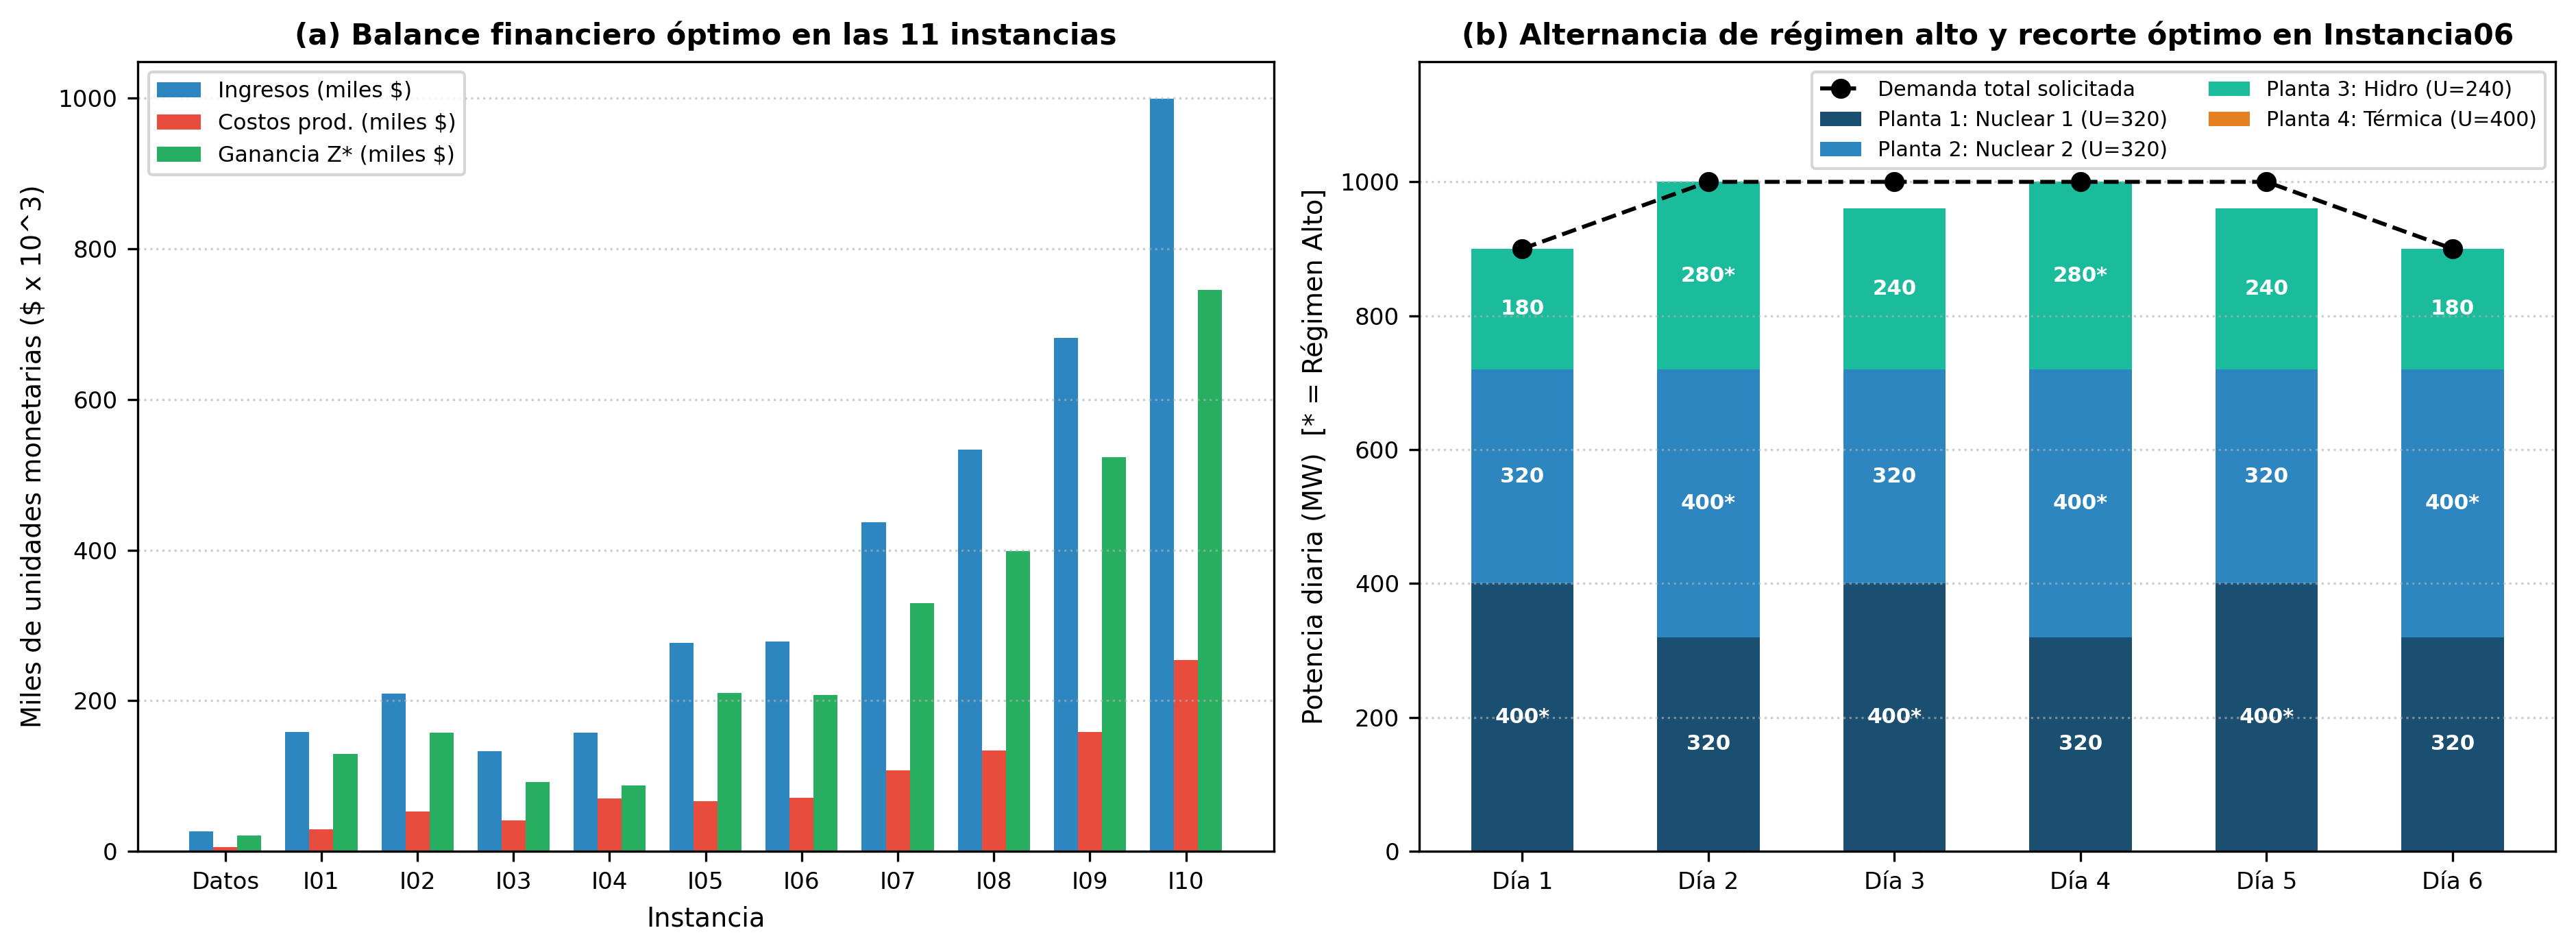
\includegraphics[width=0.98\textwidth]{1/despacho_instancias.png}
    \caption{Análisis económico-operativo de las pruebas: (a) ingresos, costos y ganancia óptima $Z^*$ en las 11 instancias; (b) despacho diario por planta en \texttt{Instancia06.dzn}, ilustrando la alternancia de régimen alto ($400^*\text{ MW}$ frente a $320\text{ MW}$) entre las dos centrales Nucleares gemelas y la Hidroeléctrica ($280^*\text{ MW}$ frente a $240\text{ MW}$).}
    \label{fig:despacho_instancias}
\end{figure}

El examen detallado de las soluciones óptimas en la Tabla~\ref{tab:resultados_instancias} y la Figura~\ref{fig:despacho_instancias}b revela tres comportamientos operativos clave:
\begin{enumerate}
    \item \textbf{Sincronización desfasada de turbinas ante la restricción de régimen alto ($C_4$):} En \texttt{Instancia06.dzn} (Figura~\ref{fig:despacho_instancias}b), las dos centrales Nucleares gemelas ($Cap_1=Cap_2=400\text{ MW}$, $U_1=U_2=320\text{ MW}$, $R_1=R_2=2$) no pueden operar dos días seguidos por encima de $320\text{ MW}$. El optimizador descubre automáticamente un patrón de relevo en contrafase: la Nuclear 1 opera en régimen alto ($400^*\text{ MW}$) en los días impares ($1, 3, 5$) y descansa exactamente en el umbral normal ($320\text{ MW}$) en los días pares ($2, 4, 6$), mientras que la Nuclear 2 descansa en $320\text{ MW}$ en los días impares y asume el régimen alto ($400^*\text{ MW}$) en los días pares. De este modo, el subparque nuclear entrega de forma constante $720\text{ MW}$ diarios a costo mínimo ($10\text{ \$/MW}$) sin infringir jamás la ventana $R_i = 2$.
    \item \textbf{Racionamiento selectivo frente a centrales de punta costosas:} En la sexta instancia (\texttt{Instancia06.dzn}), los días $2, 3, 4$ y $5$ presentan una demanda total de $1\,000\text{ MW}$. En los días $2$ y $4$, la central Hidroeléctrica ($c_3=20$, $U_3=240$, $R_3=2$) entra en régimen alto aportando $280^*\text{ MW}$ para completar los $1\,000\text{ MW}$. Sin embargo, en los días $3$ y $5$, la Hidroeléctrica está obligada a enfriarse en $240\text{ MW}$ ($720 + 240 = 960\text{ MW}$). Para cubrir los $40\text{ MW}$ restantes hacia la demanda máxima del Cliente 4 ($P_4 = 25\text{ \$/MW}$, $d_{4,3}=140$, $d^{\min}_{4,3}=70$), la única planta disponible sería la Térmica ($c_4 = 35\text{ \$/MW}$). Como $P_4 - c_4 = -10\text{ \$/MW} < 0$, el modelo mantiene apagada la Térmica ($0\text{ MW}$) y recorta en $40\text{ MW}$ la venta al Cliente 4 en los días $3$ y $5$ ($98.6\%$ de satisfacción global), ahorrando $\$800$ de pérdida operativa.
    \item \textbf{Resiliencia ante retiro de centrales:} Al eliminar la planta Nuclear en la cuarta instancia ($np=2$), las centrales Hidroeléctrica y Térmica priorizan el $100\%$ de la demanda de los Clientes 1 y 2 ($P_1=65, P_2=50 > c_T=28$) y suministran exactamente el piso legal ($G=50\%$) al Cliente 3 ($P_3=24 < c_T=28$), alcanzando $Z^* = 87\,720$ en solo $11$ nodos.
\end{enumerate}

\subsection{Análisis de Ablación: Impacto de las Restricciones Redundantes y Simetrías}

La Tabla~\ref{tab:ablacion_cop} y las Figuras~\ref{fig:arbol_bnb_cop}a y~\ref{fig:comparacion_poda_cop} cuantifican el aporte progresivo de las mejoras de modelado comparando cinco variantes acumulativas bajo la estrategia oficial $E_1$ con límite de corte de $2\,500\text{ ms}$: $M_0$ (borrador inicial con booleanas reificadas \texttt{total} y \texttt{parcial} sin redundantes), $M_1$ (modelo primario limpio $C_1$--$C_4$), $M_2$ ($M_1 + R_1 + R_2 + R_3$), $M_3$ ($M_2 + R_4 + R_5$) y $M_4$ ($M_3 + S_1 + S_2$).

\begin{table}[htbp]
    \centering
    \scriptsize
    \setlength{\tabcolsep}{1.8pt}
    \caption{Estudio de ablación ($M_0 \to M_4$): nodos explorados y propagaciones en Gecode 6.4.0 y Chuffed 0.14.0 (TO = Timeout $> 2.5\text{ s}$).}
    \label{tab:ablacion_cop}
    \begin{tabular}{lrrrrrrrr}
        \toprule
        & \multicolumn{4}{c}{Gecode 6.4.0 — Nodos (Propagaciones)} & \multicolumn{4}{c}{Chuffed 0.14.0 — Nodos (Propagaciones)} \\
        \cmidrule(lr){2-5} \cmidrule(lr){6-9}
        Instancia & $M_0 / M_1$ & $M_2$ ($+R_{1..3}$) & $M_3$ ($+R_{4..5}$) & $M_4$ ($+S_{1..2}$) & $M_0 / M_1$ & $M_2$ ($+R_{1..3}$) & $M_3$ ($+R_{4..5}$) & $M_4$ ($+S_{1..2}$) \\
        \midrule
        \texttt{Datos.dzn}       & TO & $21$ ($181$) & $1$ ($264$) & $\mathbf{1}$ ($264$) & TO & $27$ ($190$) & $1$ ($67$) & $\mathbf{1}$ ($67$) \\
        \texttt{Instancia01.dzn} & TO & $37$ ($335$) & $5$ ($464$) & $\mathbf{5}$ ($464$) & TO & $42$ ($295$) & $6$ ($161$) & $\mathbf{6}$ ($161$) \\
        \texttt{Instancia02.dzn} & TO & TO           & $48$ ($3.0\text{k}$) & $\mathbf{48}$ ($3.0\text{k}$) & TO & TO & $53$ ($1.2\text{k}$) & $\mathbf{53}$ ($1.2\text{k}$) \\
        \texttt{Instancia03.dzn} & TO & TO           & $98$ ($6.5\text{k}$) & $\mathbf{98}$ ($6.5\text{k}$) & TO & TO & $64$ ($2.4\text{k}$) & $\mathbf{64}$ ($2.4\text{k}$) \\
        \texttt{Instancia05.dzn} & TO & TO           & $199$ ($21\text{k}$) & $\mathbf{199}$ ($21\text{k}$) & TO & TO & $161$ ($12\text{k}$) & $\mathbf{161}$ ($12\text{k}$) \\
        \texttt{Instancia06.dzn} & TO & TO           & $432$ ($46\text{k}$) & $\mathbf{304}$ ($29\text{k}$) & TO & TO & $193$ ($16\text{k}$) & $\mathbf{163}$ ($13\text{k}$) \\
        \texttt{Instancia08.dzn} & TO & TO           & $3\,062$ ($481\text{k}$) & $\mathbf{3\,062}$ ($481\text{k}$) & TO & TO & $676$ ($55\text{k}$) & $\mathbf{676}$ ($55\text{k}$) \\
        \texttt{Instancia10.dzn} & TO & TO           & $143\text{k}$ ($30\text{M}$) & $\mathbf{95.8\text{k}}$ ($20\text{M}$) & TO & TO & $16.6\text{k}$ ($1.1\text{M}$) & $\mathbf{14.5\text{k}}$ ($1.2\text{M}$) \\
        \bottomrule
    \end{tabular}
\end{table}

\begin{figure}[htbp]
    \centering
    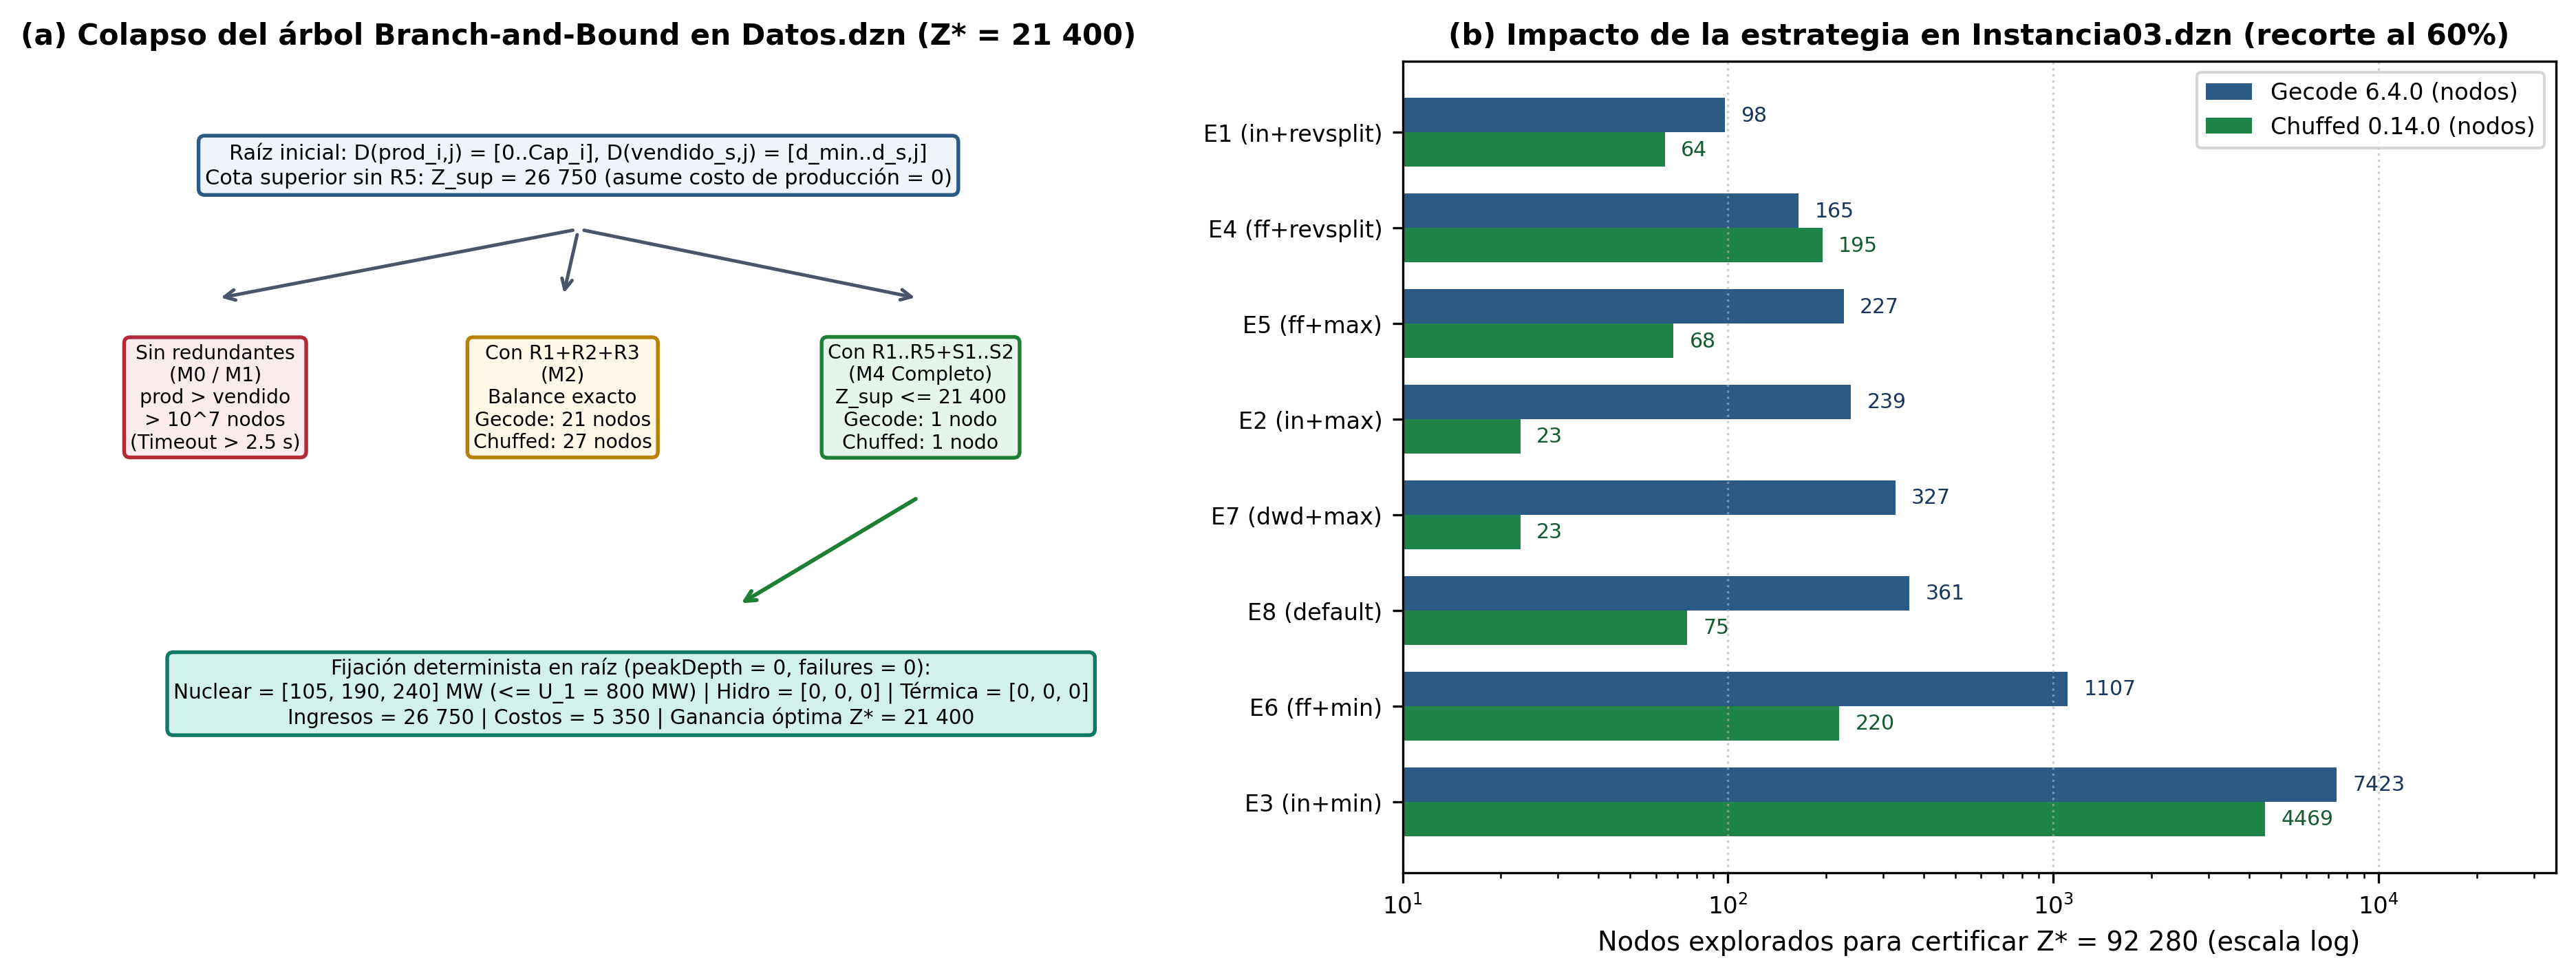
\includegraphics[width=0.98\textwidth]{1/arbol_bnb_cop.png}
    \caption{Efecto estructural de las mejoras sobre \emph{Branch-and-Bound}: (a) colapso a $1$ nodo raíz en \texttt{Datos.dzn} mediante la proyección de Fourier-Motzkin $R_5$; (b) comparación de nodos explorados por las 8 estrategias de búsqueda en \texttt{Instancia03.dzn}.}
    \label{fig:arbol_bnb_cop}
\end{figure}

\begin{figure}[htbp]
    \centering
    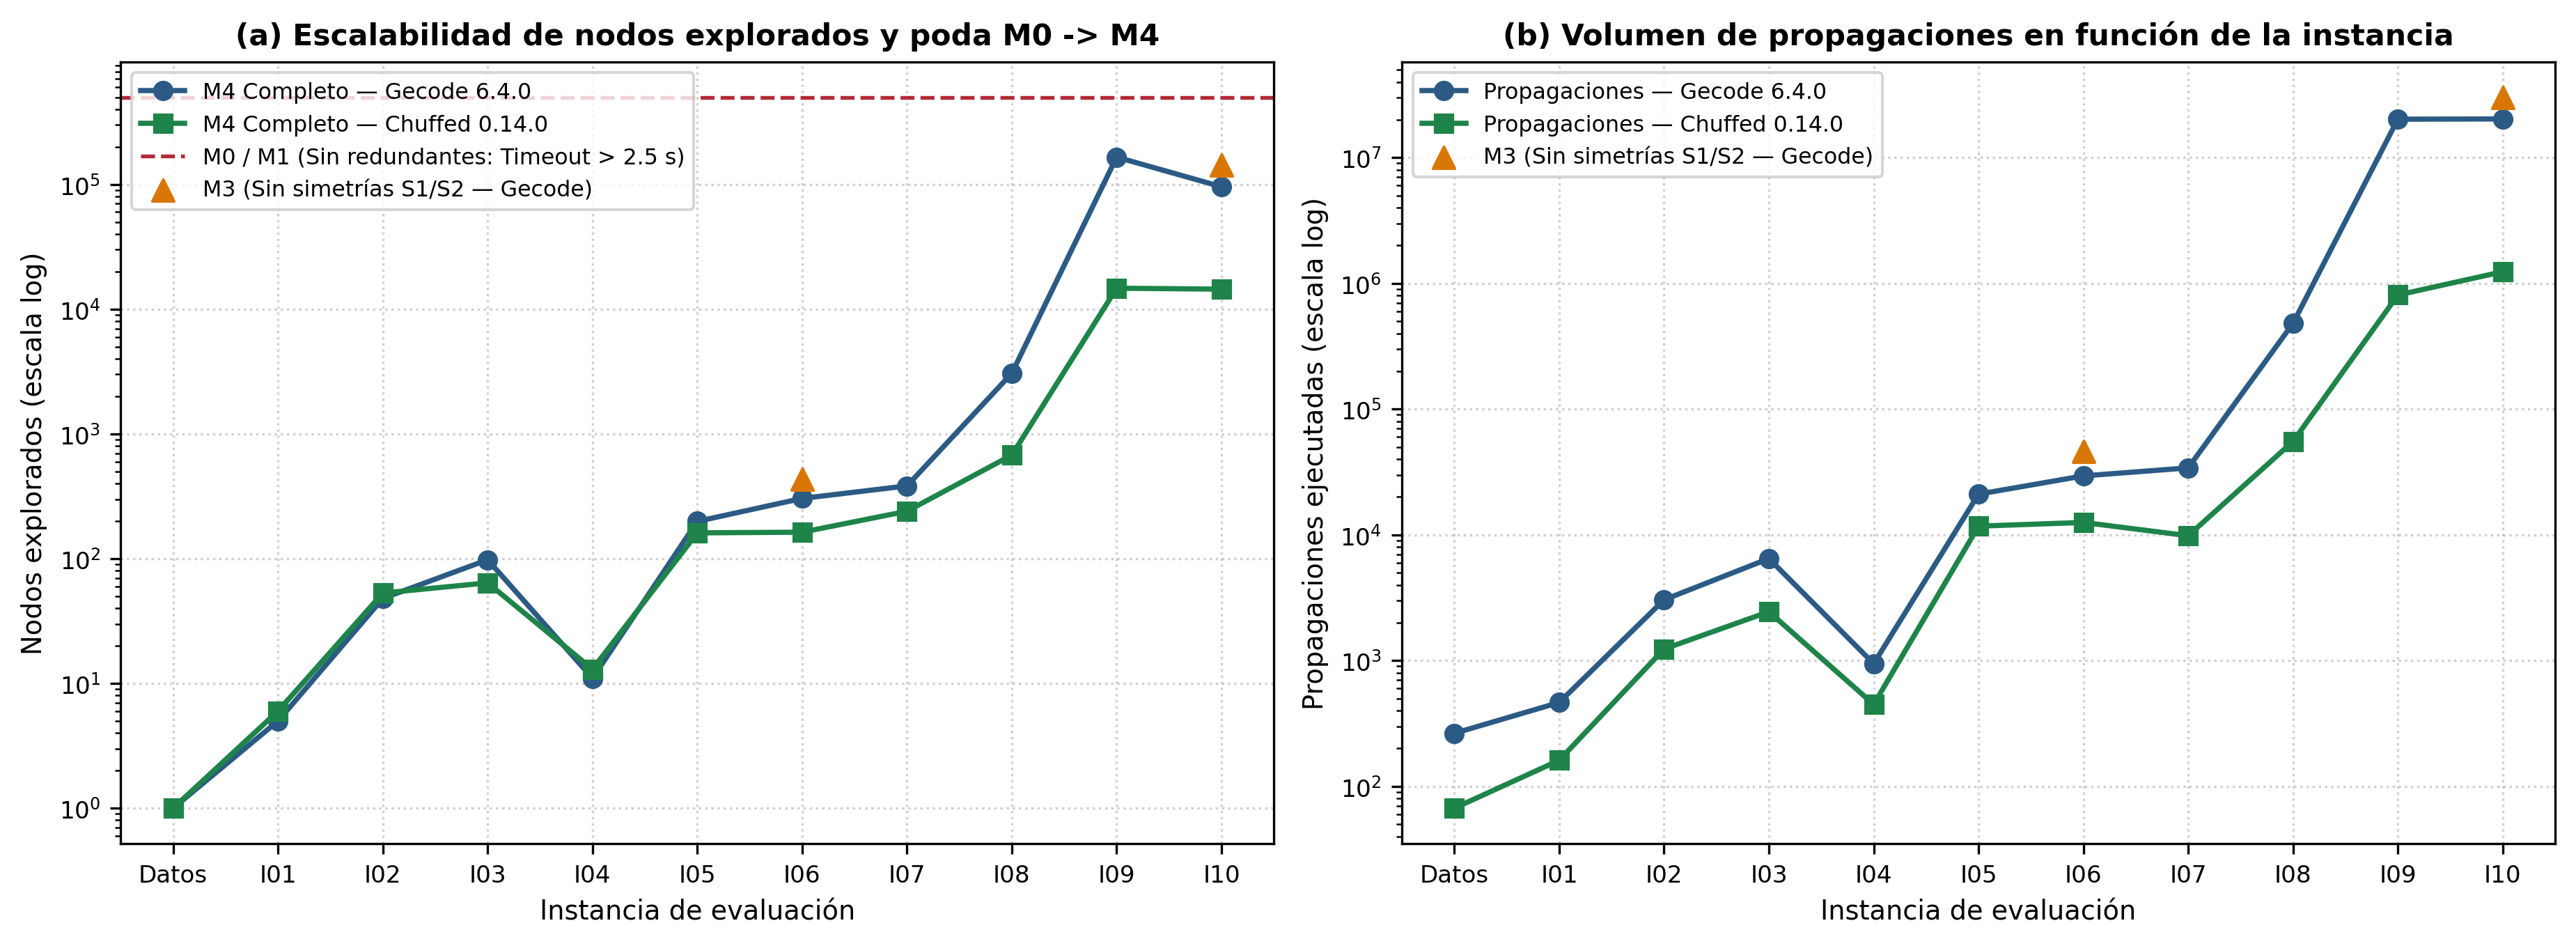
\includegraphics[width=0.98\textwidth]{1/comparacion_poda_cop.png}
    \caption{Escalabilidad del modelo completo $M_4$ frente a las variantes de ablación en las 11 instancias: (a) nodos explorados en escala logarítmica; (b) propagaciones ejecutadas por Gecode 6.4.0 y Chuffed 0.14.0.}
    \label{fig:comparacion_poda_cop}
\end{figure}

Los resultados de ablación demuestran empíricamente las propiedades teóricas deducidas en la Sección~\ref{sec:implementacion}:
\begin{itemize}
    \item \textbf{Transición de intratable ($M_0/M_1$) a resolución exacta mediante $R_1$--$R_3$ ($M_2$) y $R_4$--$R_5$ ($M_3$):} Sin la igualdad de balance diario $R_2$, tanto $M_0$ como $M_1$ exceden el tiempo límite incluso en la instancia más pequeña (\texttt{Datos.dzn}, $18$ variables), debido a la explosión combinatoria de estados con sobreproducción $\sum prod > \sum vendido$. Incorporar $R_1+R_2+R_3$ ($M_2$) resuelve \texttt{Datos.dzn} en $21$ nodos y \texttt{Instancia01.dzn} en $37$ nodos, pero resulta insuficiente cuando múltiples plantas operan en régimen alto (\texttt{Instancia02.dzn} en adelante). Al añadir la dominancia de mérito $R_4$ y las proyecciones de Fourier-Motzkin $R_5$ ($M_3$), la cota superior dual $\overline{Z}$ se cierra en el nodo raíz de \texttt{Datos.dzn} ($21 \to 1$ nodo, $0$ fallos) y permite resolver la totalidad de las 11 instancias.
    \item \textbf{Poda efectiva por rompimiento de simetrías ($M_3 \to M_4$):} En las instancias sin plantas gemelas (\texttt{Datos.dzn} a \texttt{Instancia05.dzn} e \texttt{Instancia08.dzn}), el predicado estático \texttt{where} de $S_1$ y $S_2$ se evalúa en falso durante la compilación y añade exactamente cero propagadores ($M_3 \equiv M_4$). En cambio, cuando existen plantas gemelas, $S_1$ y $S_2$ eliminan permutaciones redundantes entre filas equivalentes: en \texttt{Instancia06.dzn} (2 Nucleares gemelas) reducen los nodos de Gecode en un \textbf{$29.6\%$} ($432 \to 304$) y las propagaciones en un \textbf{$35.8\%$} ($45\,778 \to 29\,410$), mientras que en \texttt{Instancia10.dzn} (3 pares de plantas gemelas y 1 par de clientes gemelos) reducen los nodos de Gecode en un \textbf{$33.2\%$} ($143\,390 \to 95\,808$, ahorrando $9.93$ millones de propagaciones) y los de Chuffed en un \textbf{$12.8\%$} ($16\,590 \to 14\,463$).
\end{itemize}

\subsection{Comparación Experimental de las Estrategias de Búsqueda}

La Tabla~\ref{tab:estrategias_cop} y la Figura~\ref{fig:estrategias_busqueda_cop} comparan el rendimiento de las ocho estrategias de búsqueda definidas en la Sección~\ref{sec:busqueda} aplicadas sobre el modelo completo $M_4$.

\begin{table}[htbp]
    \centering
    \scriptsize
    \setlength{\tabcolsep}{0.9pt}
    \caption{Comparación estadística de las 8 estrategias de búsqueda sobre el modelo completo $M_4$ (TO = Timeout $> 2.5\text{ s}$).}
    \label{tab:estrategias_cop}
    \begin{tabular}{llrrrrrrrrrr}
        \toprule
        & & \multicolumn{5}{c}{Gecode 6.4.0 — Nodos ($t_{\text{solve}}$ ms)} & \multicolumn{5}{c}{Chuffed 0.14.0 — Nodos ($t_{\text{solve}}$ ms)} \\
        \cmidrule(lr){3-7} \cmidrule(lr){8-12}
        Cód. & Estrategia & \texttt{I02} & \texttt{I03} & \texttt{I06} & \texttt{I08} & \texttt{I10} & \texttt{I02} & \texttt{I03} & \texttt{I06} & \texttt{I08} & \texttt{I10} \\
        \midrule
        $E_1$ & \texttt{in,revsplit} & $48$ ($0.3$) & $\mathbf{98}$ ($\mathbf{0.6}$) & $\mathbf{304}$ ($\mathbf{2.1}$) & $\mathbf{3.1\text{k}}$ ($\mathbf{40}$) & $\mathbf{96\text{k}}$ ($\mathbf{1.5\text{s}}$) & $53$ ($1$) & $64$ ($1$) & $163$ ($3$) & $676$ ($14$) & $14\text{k}$ ($\mathbf{473}$) \\
        $E_2$ & \texttt{in,max}      & $\mathbf{8}$ ($\mathbf{0.1}$) & $239$ ($1.1$) & $1.4\text{k}$ ($6.1$) & $53\text{k}$ ($425$) & TO & $\mathbf{13}$ ($\mathbf{0}$) & $\mathbf{23}$ ($\mathbf{0}$) & $\mathbf{64}$ ($\mathbf{2}$) & $\mathbf{284}$ ($\mathbf{13}$) & $12\text{k}$ ($623$) \\
        $E_3$ & \texttt{in,min}      & $7.8\text{k}$ ($16$) & $7.4\text{k}$ ($17$) & $29\text{k}$ ($69$) & $303\text{k}$ ($2.0\text{s}$) & TO & $4.0\text{k}$ ($27$) & $4.5\text{k}$ ($34$) & $23\text{k}$ ($174$) & $89\text{k}$ ($868$) & TO \\
        $E_4$ & \texttt{ff,revsplit} & $69$ ($0.4$) & $165$ ($1.2$) & $3.1\text{k}$ ($12$) & $6.0\text{k}$ ($42$) & TO & $69$ ($1$) & $195$ ($3$) & $1.2\text{k}$ ($12$) & $828$ ($45$) & TO \\
        $E_5$ & \texttt{ff,max}      & $135$ ($0.6$) & $227$ ($0.8$) & $2.4\text{k}$ ($8.0$) & $24\text{k}$ ($123$) & TO & $389$ ($7$) & $68$ ($2$) & $659$ ($18$) & $1.5\text{k}$ ($88$) & TO \\
        $E_6$ & \texttt{ff,min}      & $2.8\text{k}$ ($4.9$) & $1.1\text{k}$ ($3.3$) & $8.9\text{k}$ ($28$) & $237\text{k}$ ($817$) & TO & $2.2\text{k}$ ($17$) & $220$ ($5$) & $1.1\text{k}$ ($31$) & $4.2\text{k}$ ($296$) & TO \\
        $E_7$ & \texttt{dwd,max}     & $15$ ($0.2$) & $327$ ($1.1$) & $1.0\text{k}$ ($4.2$) & $12\text{k}$ ($82$) & TO & $\mathbf{13}$ ($\mathbf{0}$) & $\mathbf{23}$ ($1$) & $\mathbf{64}$ ($5$) & $\mathbf{284}$ ($15$) & $12\text{k}$ ($568$) \\
        $E_8$ & \texttt{default}     & $1.7\text{k}$ ($3.1$) & $361$ ($1.2$) & $3.4\text{k}$ ($8.3$) & $39\text{k}$ ($235$) & TO & $102$ ($2$) & $75$ ($2$) & $190$ ($8$) & $534$ ($36$) & $\mathbf{4.0\text{k}}$ ($535$) \\
        \bottomrule
    \end{tabular}
\end{table}

\begin{figure}[htbp]
    \centering
    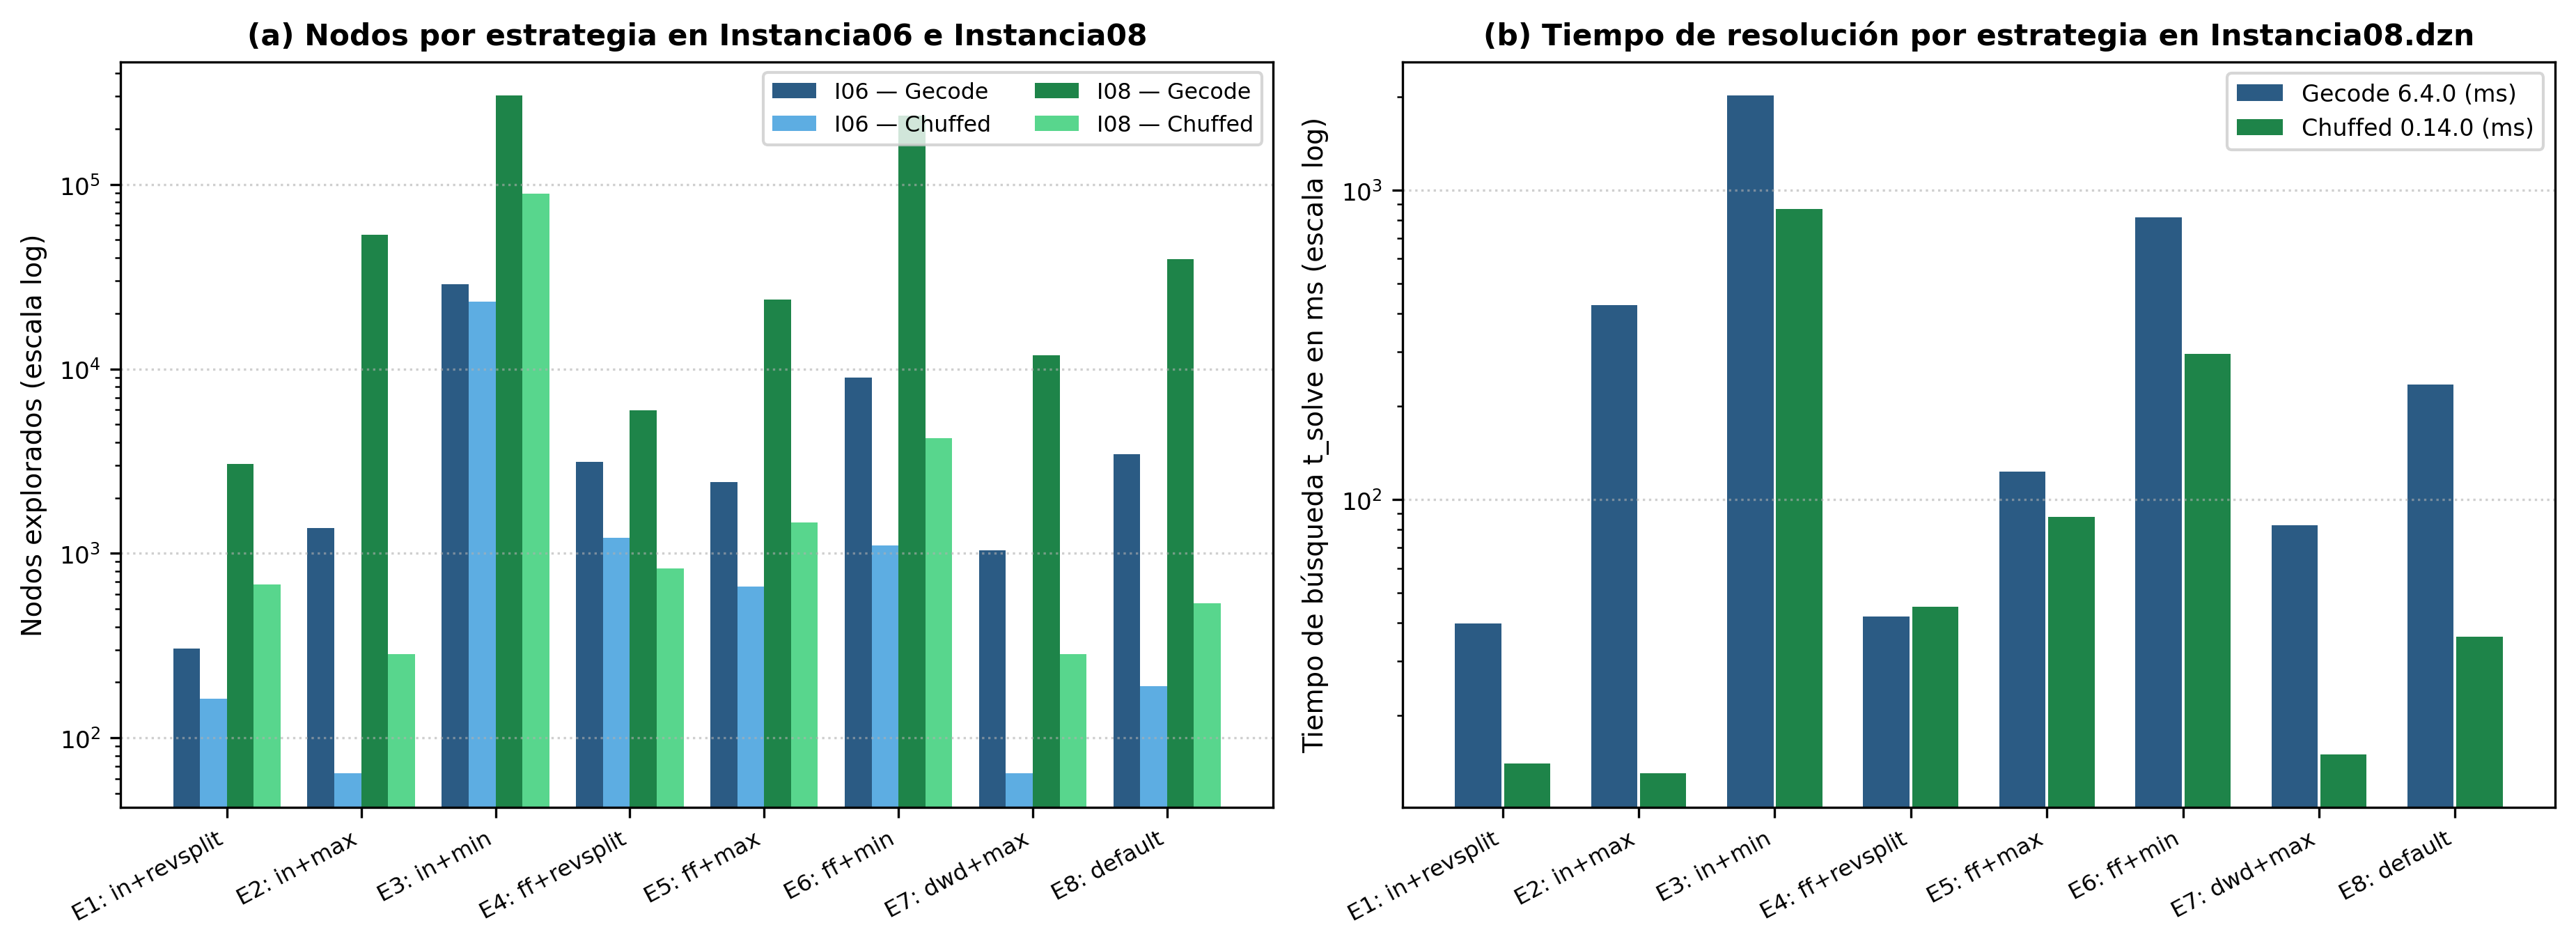
\includegraphics[width=0.98\textwidth]{1/estrategias_busqueda_cop.png}
    \caption{Desempeño comparativo de las 8 estrategias de búsqueda ($E_1$--$E_8$): (a) nodos explorados en \texttt{Instancia06.dzn} e \texttt{Instancia08.dzn}; (b) tiempos de resolución $t_{\text{solve}}$ (ms) en \texttt{Instancia08.dzn}.}
    \label{fig:estrategias_busqueda_cop}
\end{figure}

La evidencia experimental de la Tabla~\ref{tab:estrategias_cop} y la Figura~\ref{fig:estrategias_busqueda_cop} confirma de forma contundente la teoría expuesta en la Sección~\ref{subsec:teoria_busqueda}:
\begin{itemize}
    \item \textbf{Robustez y escalabilidad superior de $E_1$ (orden de entrada con bisección descendente):} $E_1$ es la \textbf{única estrategia de las ocho evaluadas} capaz de resolver la totalidad de las 11 instancias hasta optimalidad certificada dentro del límite de tiempo en ambos motores (\texttt{Instancia10.dzn}: $95\,808$ nodos y $1.48\text{ s}$ en Gecode; $14\,463$ nodos y $0.47\text{ s}$ en Chuffed). En \texttt{Instancia08.dzn} bajo Gecode, $E_1$ ($3\,062$ nodos, $39.8\text{ ms}$) reduce los nodos en un factor de \textbf{$17.4\times$} frente a la enumeración unitaria descendente $E_2$ ($53\,167$ nodos, $425.5\text{ ms}$), en \textbf{$12.8\times$} frente a la búsqueda por defecto $E_8$ ($39\,337$ nodos), en \textbf{$77.3\times$} frente a la estrategia del borrador inicial $E_6$ ($236\,811$ nodos) y en \textbf{$99.0\times$} frente a $E_3$ ($303\,157$ nodos, $2\,022.6\text{ ms}$).
    \item \textbf{Ventaja de \texttt{input\_order} ($prod \to vendido$) frente a \texttt{first\_fail}:} Comparando a igualdad de selector de valor ($E_1$ frente a $E_4$, y $E_2$ frente a $E_5$), \texttt{input\_order} supera sistemáticamente a \texttt{first\_fail} en \texttt{Instancia06.dzn} ($304$ frente a $3\,128$ nodos en Gecode; $163$ frente a $1\,219$ en Chuffed) y en \texttt{Instancia10.dzn} (donde todas las variantes con \texttt{first\_fail}, $E_4$--$E_6$, sufren \emph{timeout} en ambos motores). Ello verifica que preservar el orden causal de decisión (primero la trayectoria de las centrales por orden de mérito y después la asignación comercial a clientes) evita ramificar prematuramente sobre los dominios estrechos de $vendido_{s,j}$.
    \item \textbf{Sinergia entre aprendizaje de cláusulas (Chuffed) y selección de valor máximo ($E_2, E_7$):} Mientras que Gecode requiere bisección de intervalos ($E_1$) para no degradarse en escalones de capacidad grandes, Chuffed representa internamente los enteros mediante literales booleanos de cota $[\![ x \le v ]\!]$ y aprende cláusulas de conflicto (\emph{nogoods}) que saltan directamente desde $Cap_i$ hasta el umbral $U_i$ en un solo \emph{backjump}. Gracias a ello, en Chuffed las estrategias $E_2$ y $E_7$ resuelven \texttt{Instancia03.dzn}, \texttt{Instancia06.dzn} e \texttt{Instancia08.dzn} en apenas $23$, $64$ y $284$ nodos respectivamente.
\end{itemize}
